{\color{indiagreen}\subsection{Enakomerno pospešeno gibanje}}
Enakomerno pospešeno gibanje je gibanje pri katerem se hitrost \textbf{enakomerno spreminja}. Pospešek nam pove za koliko se v določenem času spremeni hitrost.\\
$\frac{\frac{m}{s}}{s}\rightarrow \quad [\frac{m}{s^2}] \rightarrow \quad enota$\\
\begin{align*}
	a &= \frac{\Delta v}{ \Delta t}\\
\end{align*}
\textbf{GRAFI:}\\
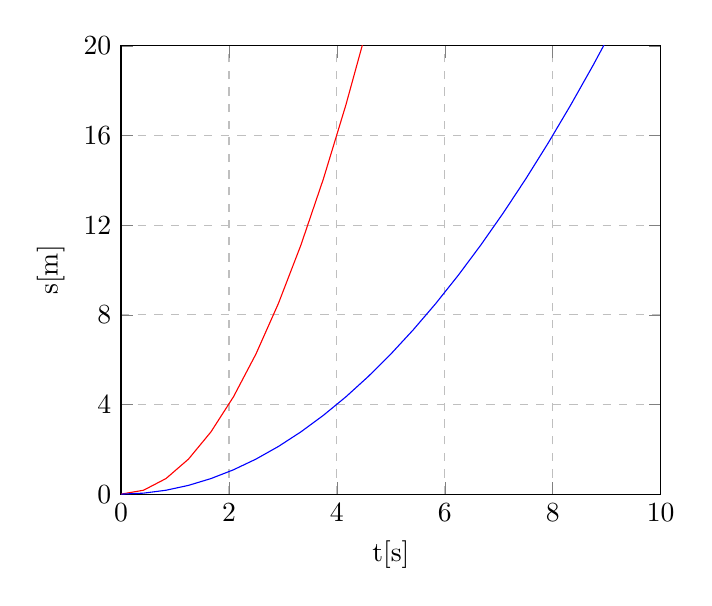
\begin{tikzpicture}
\begin{axis}[
    xlabel={t[s]},
    ylabel={s[m]},
    xmin=0, xmax=10,
    ymin=0, ymax=20,
    xtick={0,2,4,6,8,10},
    ytick={0,4,8,12,16,20},
    ymajorgrids=true,
    xmajorgrids=true,
    grid style=dashed,
]
 
\addplot[domain=0:10,red] {x^2};
\addplot[domain=0:10,blue] {(x/2)^2};
 
\end{axis}

\end{tikzpicture}
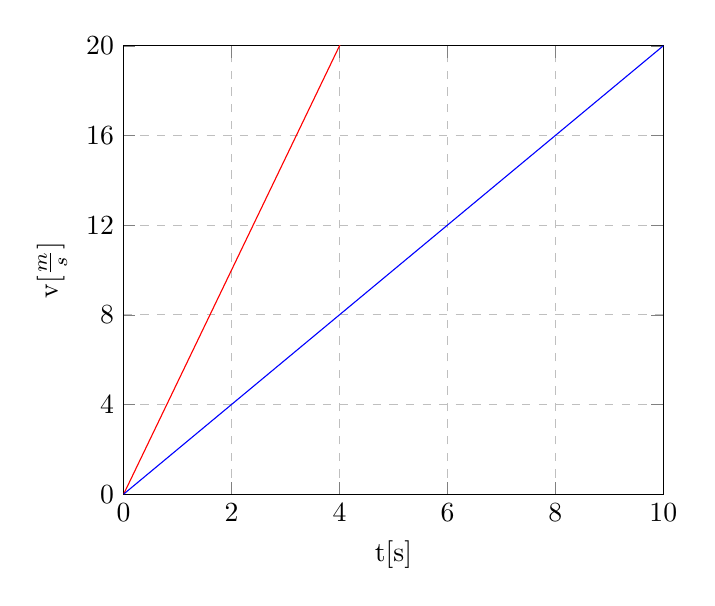
\begin{tikzpicture}
\begin{axis}[
    xlabel={t[s]},
    ylabel={v[$\frac{m}{s}$]},
    xmin=0, xmax=10,
    ymin=0, ymax=20,
    xtick={0,2,4,6,8,10},
    ytick={0,4,8,12,16,20},
    ymajorgrids=true,
    xmajorgrids=true,
    grid style=dashed,
]
 
\addplot[domain=0:10,red] {5*x};
\addplot[domain=0:10,blue] {2*x};
 
\end{axis}
\end{tikzpicture}


\begin{tikzpicture}
\begin{axis}[
    xlabel={t[s]},
    ylabel={a[$\frac{m}{s^2}$]},
    xmin=0, xmax=10,
    ymin=0, ymax=20,
    xtick={0,2,4,6,8,10},
    ytick={0,4,8,12,16,20},
    ymajorgrids=true,
    xmajorgrids=true,
    grid style=dashed,
]
 
\addplot[
    color=red,
    ]
    coordinates {

    (0,15)(10,15)
    };
\addplot[
	name path=odkje,
    color=blue,
    ]
    coordinates {
    (0,10)(10,10)
    };
    \path[name path=dokam] (axis cs:0,0) -- (axis cs:10,0);

    \addplot [
        thick,
        color=blue,
        fill=blue, 
        fill opacity=0.5
    ]
    fill between[
        of=odkje and dokam,
        soft clip={domain=0:10},
    ];
 
\end{axis}
\end{tikzpicture}

Strmina premice hitrosti od časa nam pove velikost pospeška.\\

\begin{align*}
	k &= \frac{\Delta v}{\Delta t} = a\\
\end{align*}

Tangenta na krivuljo grafa poti od časa v vsaki točki govori o hitrosti telesa.Ploščina pod krivuljo grafa pospeška od časa nam pove hitrost.\\

\begin{align*}
	v &= a * t\\
\end{align*}

Odvod poti proti času in odvod hitrosti po času\\
\begin{empheq}[box=\fbox]{align*}
  {\color{bostonuniversityred}{v}} &= {\color{bostonuniversityred}{\frac{d s}{d t}}}\\
  {\color{bostonuniversityred}{v}} &= {\color{bostonuniversityred}{\frac{d v}{d t}}}\\
\end{empheq}